\section{Methods}
\numberwithin{equation}{section}
In this section, the basic algorithm is used to demonstrate
program flow and memory hierarchy. The algorithm will be incrementally improved
by first parallelizing it on accelerator cards, and later adding several
techniques to improve sampling precision as well as runtime behaviour.

All plots and graphics in this section are based on the simulation of a single
timestep using the same gain medium (similar to
Figure~\ref{graphic:samples_reduced}) and stimulus with the following
properties:
\\
\\
\begin{tabular}{| l | l |}
\hline
Points per plane        & 321\\
\hline
Sample points           & 3210\\
\hline
Planes                  & 10\\
\hline
Triangles               & 600\\
\hline
Prisms                  & 5400\\
\hline
Height                  & 0.6 cm\\
\hline
Surface area            & 4 x 4 cm\\
\hline
Material                & $\text{Yb}^{3+}$:YAG\\
\hline
Crystal doping          & $2at.\%$\\
\hline
Spectrum                & Monochromatic\\
                        & $~\lambda = 1030nm$\\
                        & $\sigma_e = 2.4 \cdot 10^{-20}~cm^2$\\ 
                        & $\sigma_a = 1.10 \cdot 10^{-21}~cm^2$\\
\hline
\end{tabular}

\subsection{Program flow}
\label{subsec:program_flow}
\begin{figure}[H]
  \centerline
  {\resizebox{0.5\textwidth}{!}{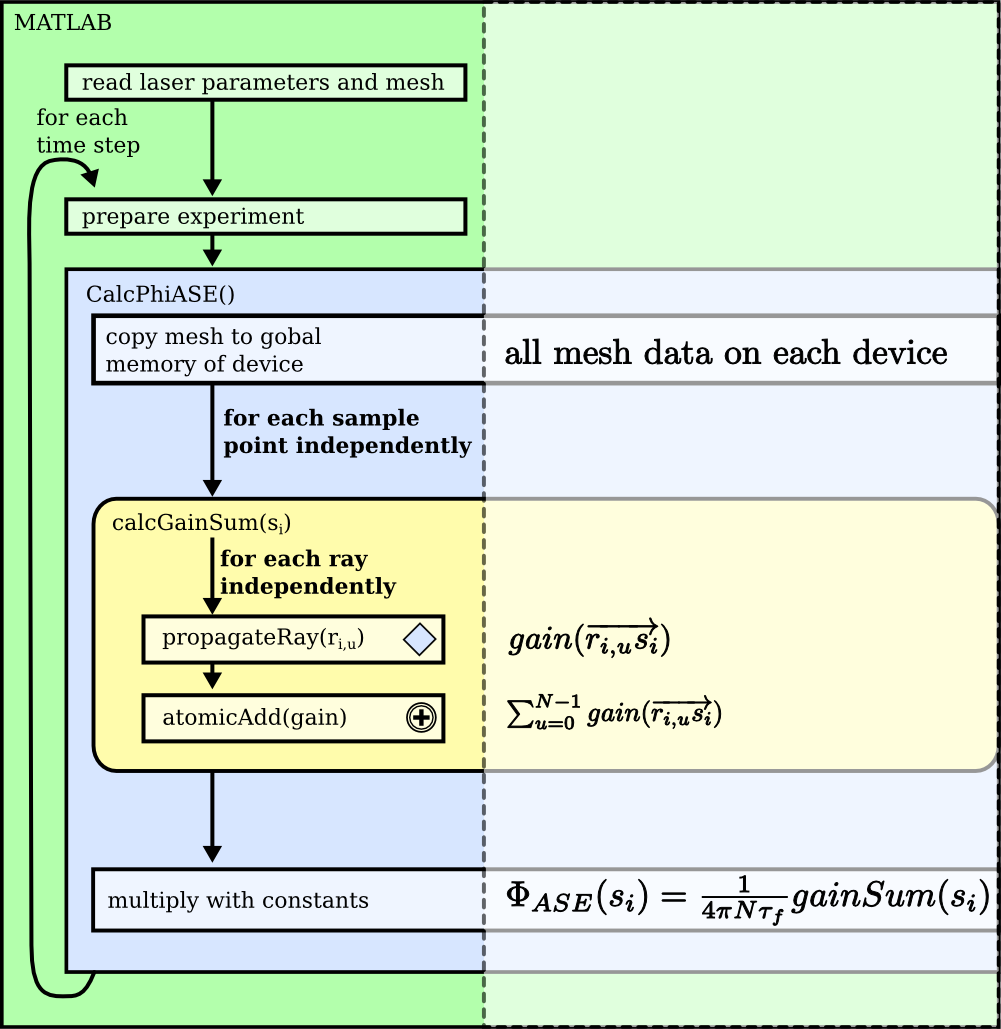
\includegraphics{graphics/PAP_step1_2.png}}}
  \caption{Basic program flow: MATLAB calls the C-application in a loop to
  simulate the timesteps. The C-application calls multiple GPU functions}
  \label{graphic:pap1}
\end{figure}
The basic programm flow (see Figure~\ref{graphic:pap1}) starts
by passing the prepared experiment data from MATLAB \cite{matlab}
to the C-application (CalcPhiASE). All information about the mesh is then copied
to the accelator card's memory and processed like described in 
the section \nameref{subsubsec:rays}. When the computation succeeds, 
all data is passed back to MATLAB and the outer loop will proceed 
with the next timestep. 

\subsection{Parallel methods}
\label{subsec:parallel_methods}
Moving from a single CPU to a multiple
GPU implementation is not so much about changing the overall algorithm,
but more about efficient utilization of the GPU resources. 
By using CUDA\cite{cuda} as a parallel computing platform created by NVIDIA\cite{nvidia},
it is possible to obtain high performance with a high level 
programming model (similar to~C). Therefore the parallelization was pushed on CUDA-thread, 
CUDA-block and multiple GPU level to reach a good speedup compared to 
the sequential implementation. 

Figure~\ref{graphic:pap1} already displays two embarrasingly parallel spots
which can be exploited. Firstly, calculation of each ray for a single sample
point is completely independent. Secondly, each sample point itself is
independent from all other sample points. 
In the following, the underlying memory hierarchy, the used parallelization
techniques and their implementations are explained.

\subsubsection{Memory hierachy}
Memory on accelerator cards in general can be split
in 3 classes: 
\begin{description}
  \item[Global memory] several gigabytes, high latency and bandwidth, global access for threads from all CUDA-blocks
  \item[Shared memory] several kilobytes, medium latency, access by threads of one CUDA-block
  \item[Global memory] several 32 bit registers, no latency, exclusive access of one thread
\end{description}
Thus, a high-performance application always involves using
a sophisticated memory hierachy that provides data by
the time it is needed for calculation.

All used data structures are one-dimensional 
arrays that are accessible through programmer-friendly interfaces to avoid
explicit pointer arithmetic.
In particular, the mesh consists of an array of points and an array of the indices
to these points. Three of these indices shape a triangle.
For the intersection and raystracing algorithms, normals and neighbors
of all edges are also included. 

The required memory for thousands or millions of rays (each ray 4 byte)
consumes the biggest amount of global memory so far, thereby setting 
a limit for simulation resolution. 

It is not possible to store all mesh data in the small register
memory, hence the mesh is stored in global memory and will
be transfered prism by prism into the registers of the
CUDA-threads (see Figure~\ref{graphic:memory_hierarchy}) when needed.

\begin{figure}[H]
  \centerline
  {\resizebox{0.5\textwidth}{!}{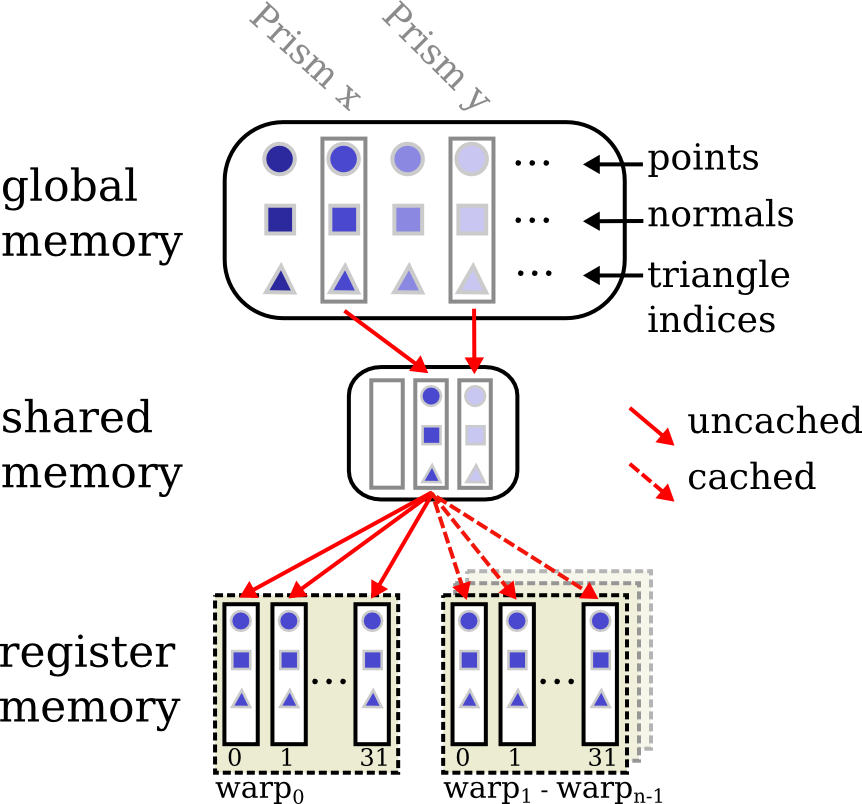
\includegraphics{graphics/memory_hierarchy.png}}}
  \caption{memory hierachy for a single CUDA-block}
  \label{graphic:memory_hierarchy}
\end{figure}
Because the trace of rays can not be predicted in advance,
the shared memory acts as L1 cache, caching
prisms from global memory to share these prisms 
with several warps.
Rays with same start prism and therefore similar trace through 
the mesh are grouped in CUDA-blocks. Thus, warps in the same block can 
reuse cached prism data from their shared memory.

\subsubsection{Rays as GPU threads}
\label{subsubsec:rays}
\begin{figure}[H]
  \centerline
  {\resizebox{0.5\textwidth}{!}{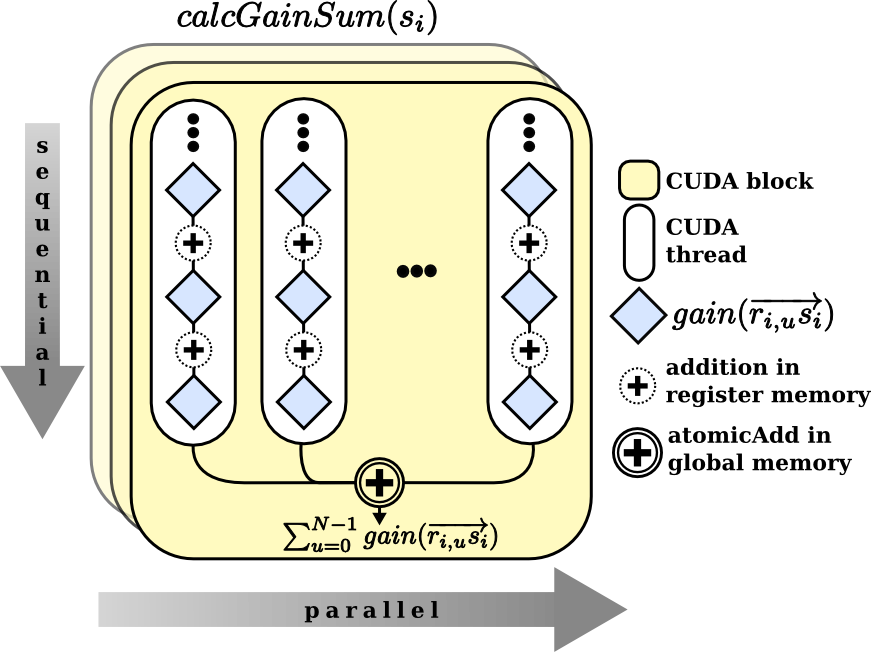
\includegraphics{graphics/kernel_detail5.png}}}
  \caption{one of 200 CUDA threadblocks to calculate $\Phi_{ASE}$}
  \label{graphic:kernel}
\end{figure}
    The raytracing of every ray can be done independently through the mesh
    structure.  Exploiting this parallelism provides a great opportunity to
    boost performance. Figure~\ref{graphic:kernel} demonstrates the distribution
    of rays. For each sample point~$s_i$, a kernel consisting of a grid of 
    maximal 200 CUDA blocks is spawned. Each of those blocks contains 128 CUDA threads.
    The maximum amount of used blocks is bounded by the used
    mersenne twister implementation~\cite{mersenne_twister} as random number generator.
    The number of threads per block was determined by the CUDA Occupancy 
    Calculator~\cite{occupancy_calculator} with the objective to obtain the
    maximum number of concurrently executed operations for the used hardware
    (see \cref{subsec:testingEnvironment}).
    
    Dependendent on the used GPU, $B$ blocks can be spawned
    in parallel on a device and since there are $N$ rays to calculate for each sample point, each thread
    traces up to $t = \lceil\frac {N}{B\cdot128}\rceil$ rays and computes the
    corresponding gain values using the following cycle (see Figure~\ref{graphic:algorithm_steps}):
    
    \begin{enumerate}
      \item Get current sample point $s_i$
      \item Request a prism $x$ to start ray from
      \item Generate start point $r_{i,u}$ inside this prism 
      \item Generate ray $\overrightarrow{r_{i,u}s_i}$
      \item Calculate the partial gains for $\overrightarrow{r_{i,u}s_i}$:
        \begin{enumerate}
          \item find intersection between $\overrightarrow{r_{i,u}s_i}$
            and $x$\label{5a}
          \item calculate length $l_x$ of partial ray $\overrightarrow{r_{i,u}r_x}$
          \item calculate $partial\_gain(x)$~\eqref{eq:partial_gain}
          \item if the ray did not reach $s_i$, determine neighboring prism $x'$,
            set $x := x'$, set $r_x$ as the new start point and repeat the 
            previous steps~\ref{5a} to~\ref{5d}.
            \label{5d}
        \end{enumerate}
      \item Calculate $gain(\overrightarrow{r_{i,u}s_i})$~\eqref{eq:gain}
      \item Add gain to gain of the other rays in the thread
    \end{enumerate}
    After a maximum of $t$ iterations, the thread has computed its share and
    adds its locally accumulated gain to the results of the other threads in a
    global reduce operation. This reduce is implemented as a sequential
    atomicAdd operation on the GPU~\eqref{eq:monte_carlo_ase}.

\begin{figure}[H]
  \centerline
  {\resizebox{0.45\textwidth}{!}{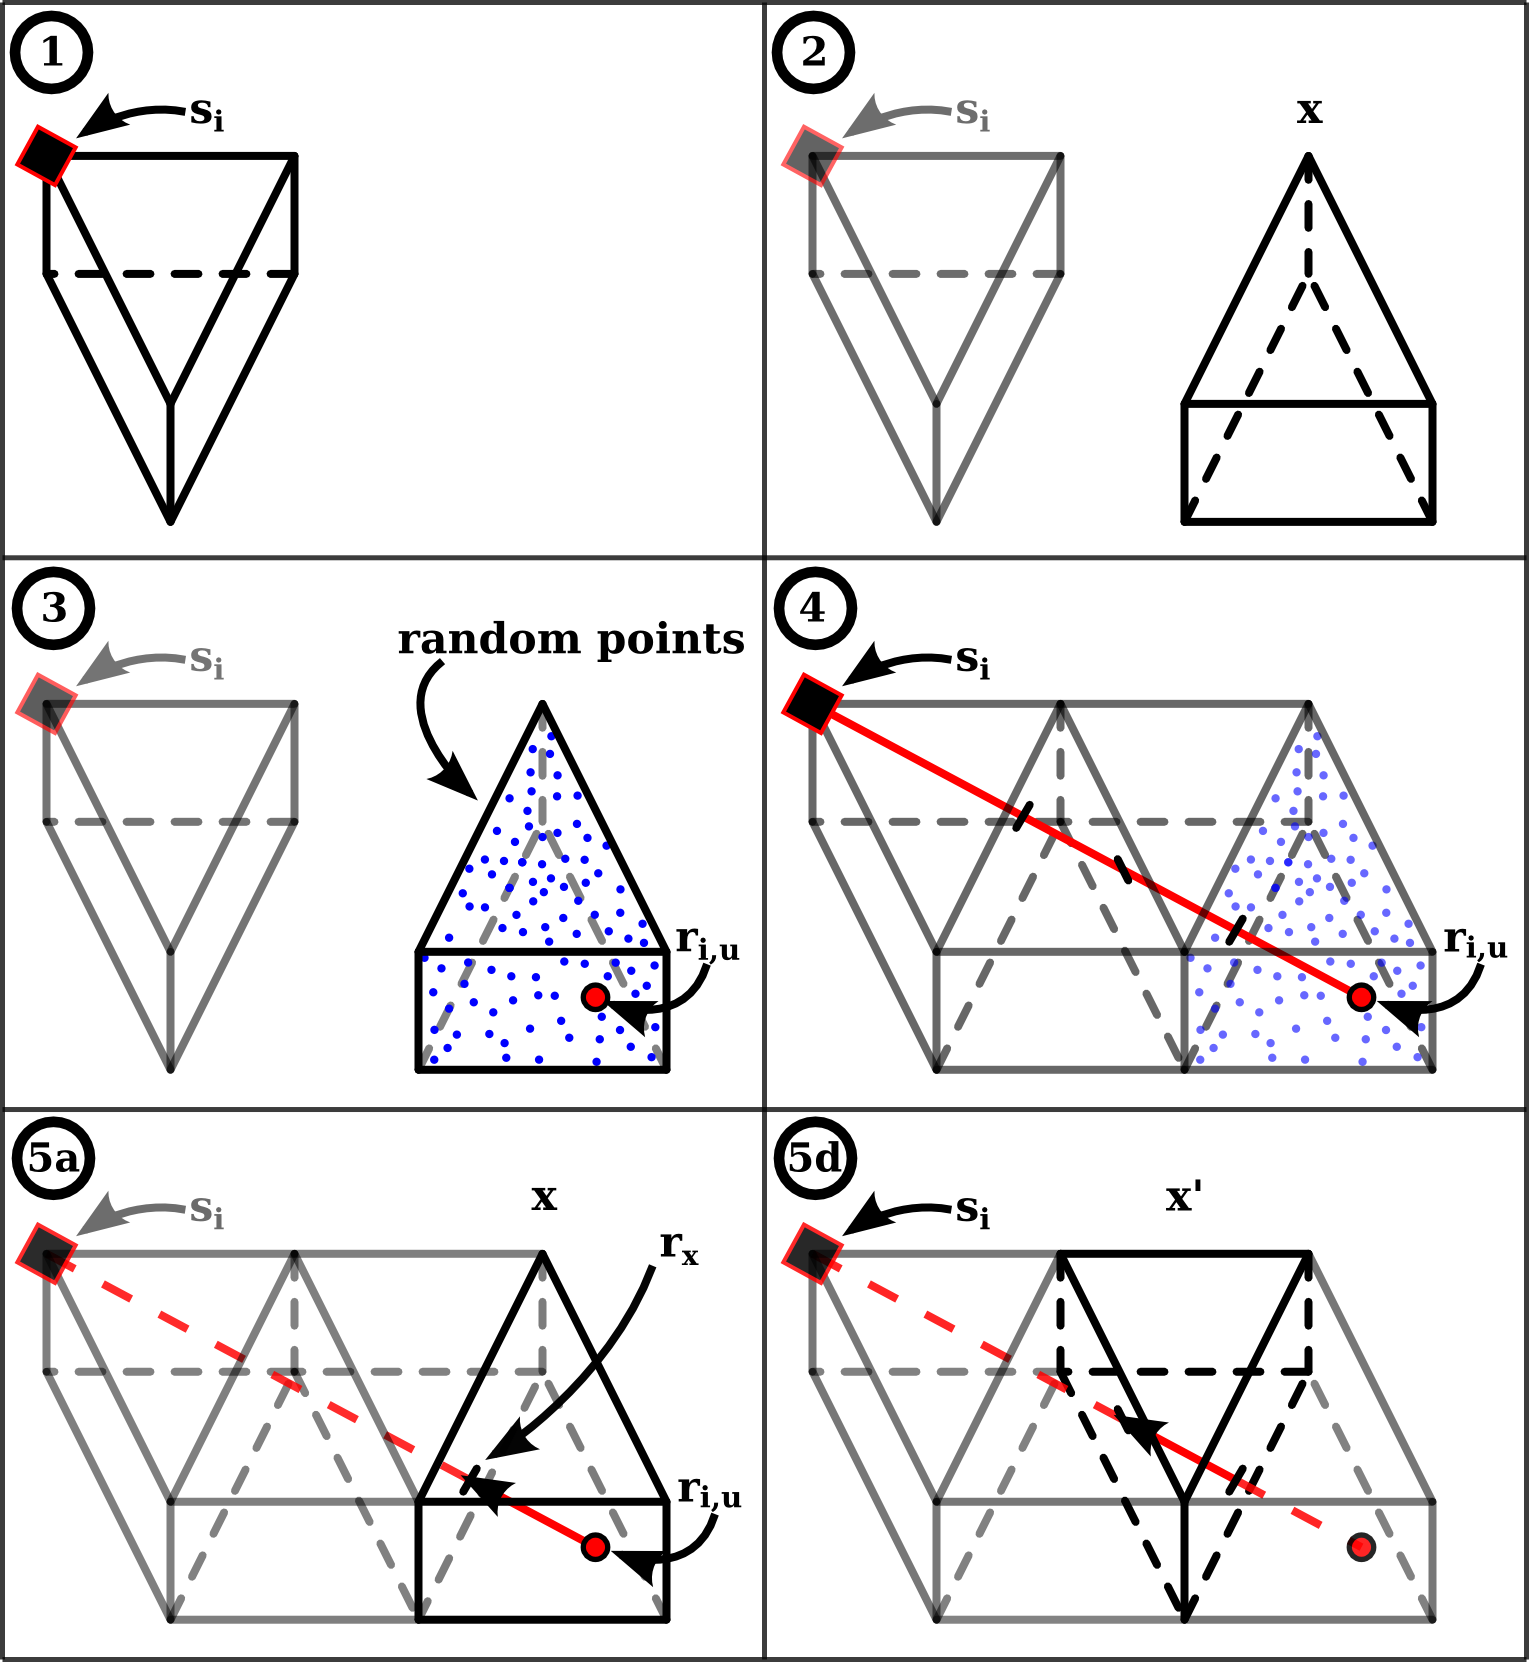
\includegraphics{graphics/iteration_detail4.png}}}
  \caption{steps for a single ray within a CUDA thread, corresponding to
  $propagate\_ray(r_{i,u})$ from Figure~\ref{graphic:pap1}}
  \label{graphic:algorithm_steps}
\end{figure}
Successive threads start rays from a similar origin, which results
in similar paths through the mesh structure and therefore often the same prisms. This
leads to better utilization of the GPU L1 cache and higher performance.

Since each distinct ray potentially has a different path through the gain
medium, the execution times between some threads will differ substantially. In case
of a static mapping from threads to rays (i.e.\ strided access), one thread can
end up calculating many rays with long paths. If there are still many of those
rays remaining, the thread has to continue working for a long time, while all
other threads are already finished. These idle threads are unable to
participate, leaving many resources on the device unused.

To improve load balancing between the threads, each thread block fetches a
workload equal to its size and executes it completely before determining a new
workload. Therefore, if a single thread calculates a ray with a very long path,
only threads in the same block depend on the duration of this long ray.
Meanwhile, threads in other blocks can pick up more work. Thus, most resources
can contribute to the computation.
    
\subsubsection{Sample Points on multiple GPUs}
\label{subsubsec:multigpu}
\begin{figure}[H]
  \centerline
  {\resizebox{0.45\textwidth}{!}{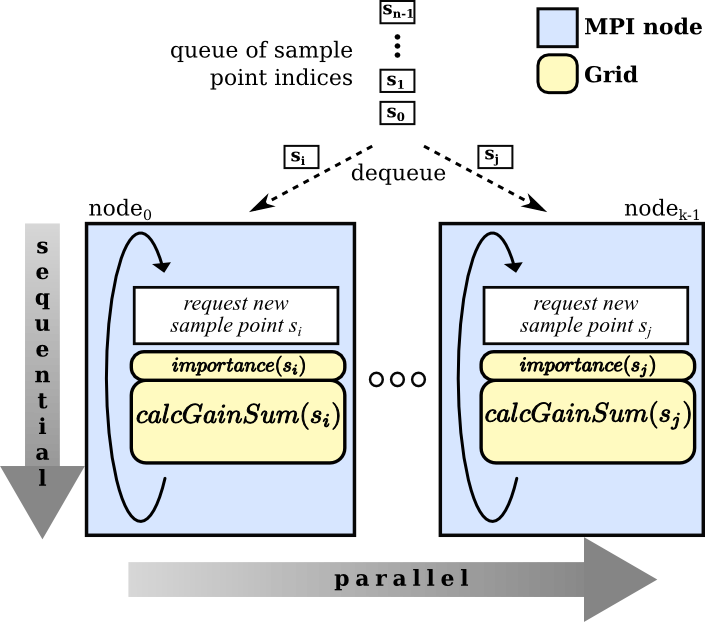
\includegraphics{graphics/multigpu_partitioning5.png}}}
  \caption{partitioning of the workload to multiple devices. All nodes store the whole mesh in
  global memory.}
  \label{graphic:multigpu}
\end{figure}
Each Monte-Carlo experiment (see \cref{eq:monte_carlo_ase}), calculates
the $\Phi_{ASE}(s_i)$ value of a sample point~$s_i$ independently from each
other. Thus, every $calcGainSum(s_i)$ calculation is executed as a
self-contained grid and therefore sample points can be distributed to
several devices.

Consider an MPI\cite{MPI} environment with $k$ nodes, each hosting 1 GPU\@. Furthermore, one
node is used as a \emph{headnode} responsible for distributing the workload. The
headnode holds a queue of all sample points. Each node requests a new sample
point and begins the calculation. As soon as the calculation is finished, a node
is able to request new work indepently from the other nodes (Figure~\ref{graphic:multigpu}). This form of load balancing is especially important in a
scenario with varying workloads for each sample point (see
\cref{subsec:adaptive_sampling}).

As a result, the speedup is almost linear in the number of GPUs. This was
verified with up to 64 nodes.
    
\subsection{Importance sampling (IS)}
\label{subsec:importance_sampling}
\begin{figure}[H]
  \centerline
  {\resizebox{0.5\textwidth}{!}{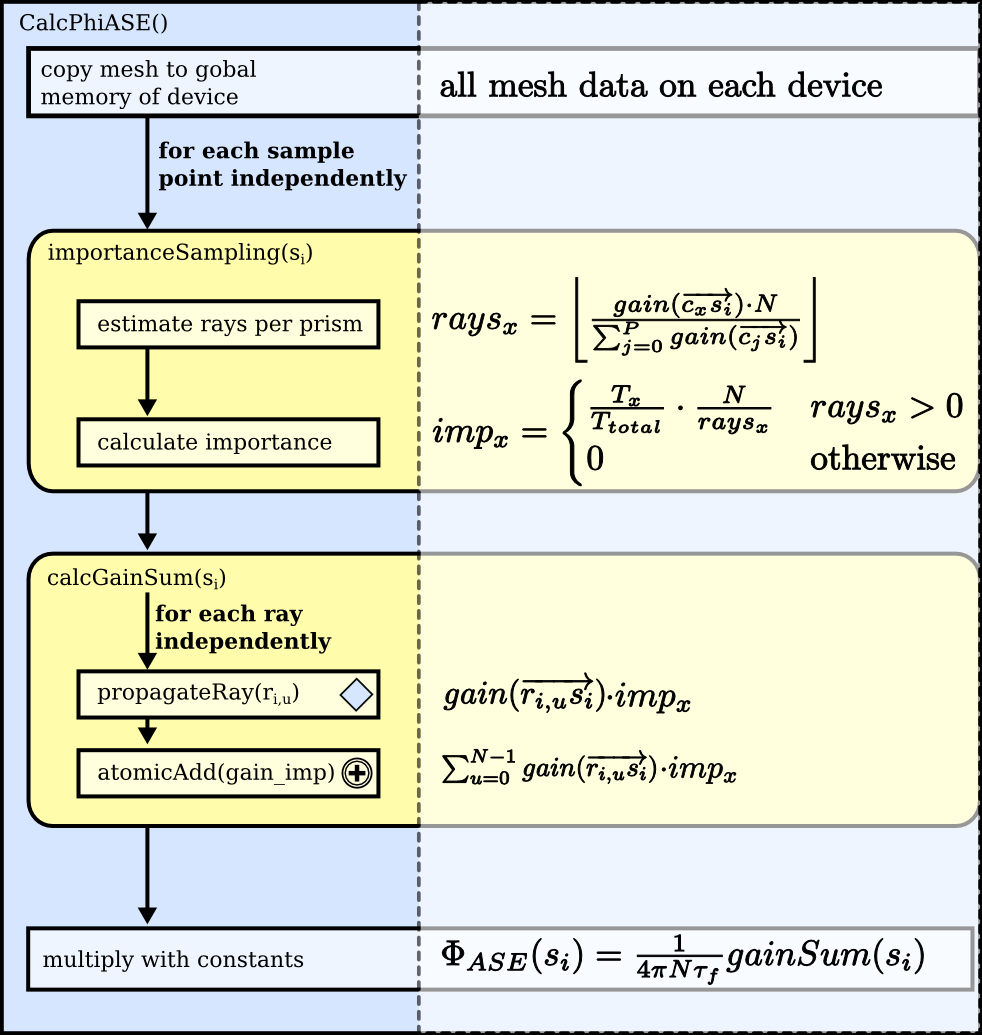
\includegraphics{graphics/PAP_step2_3.png}}}
  \caption{After adding the importance sampling, the calculated importance 
  influences the gain calculation}
  \label{graphic:pap2}
\end{figure}
Importance sampling is a well known technique in the domain
of statistics~\cite{importanceSamplingSource}. It has to be determined for each
sample point before its $\Phi_{ASE}$ calculation (see Figure~\ref{graphic:pap2},
Figure~\ref{graphic:multigpu}) and is used 
to decide which areas will have the most influence on the result.

The objective is to distribute N rays to P prims of the active gain medium, 
where areas with more influence will receive more rays.
This is done by introducing a center point~$c_x$ and triangle surfaces~$T_x$ for
every prism~$x$ with $x \in \{0,\dots,P-1\}$.
The rays per prism~$rays_x$ correlates to the expected gain for~$x$:
\begin{align}
  rays_x       &= \left\lfloor\frac{gain(\overrightarrow{c_xs_i}) \cdot N}{\sum^{P-1}_{j=0} gain(\overrightarrow{c_js_i})}\right\rfloor
\end{align}
To compensate varying values of$rays_x$, importance $imp_x$ is used as a weighting factor
and extends \eqref{eq:gain} to \eqref{eq:gain_imp}.
\begin{align}
imp_x &= 
\begin{cases}
\frac{T_x}{T_{total}} \cdot \frac{N}{rays_x} &rays_x > 0\\
0 &\text{otherwise}
\end{cases}
\end{align}
\begin{align}
\label{eq:gain_imp}
gain\_imp(\overrightarrow{r_{i,u,x}s_i})        &= gain(\overrightarrow{r_{i,u}s_i}) \cdot imp_x
\end{align}
The result of the importance sampling is a schedule for~$s_i$, that
describes in which prism each ray starts.
This method has a strong impact on the precision of the simulation
and is able to reduce strong peaks in Monte Carlo simulations.

To show the impact of importance sampling in $\Phi_{ASE}(s_i)$, the difference
\[\Phi_{ASE\Delta} = |\Phi_{ASE~IS}(M) - \Phi_{ASE~Uniform}(N)|\] of the 
result with importance sampling ($IS$) and with uniform sampling ($Uniform$) was calculated with 
$N,M = 10^5$ rays per sample point (see Figure~\ref{graphic:importance}). 
Then, N was increased two times by a factor of 10 for the simulation with uniform sampling, resulting in sampling with $10^6$ and $10^7$ rays.
The more rays are simulated, the smaller $\Phi_{ASE\Delta}$ becomes, which 
means that the simulation
with importance sampling achieves the same results with less
rays per sample point. Thus, importance sampling can increase the
efficiency of Monte Carlo simulations by reducing variance 
and simulation runtime. 
\begin{figure}[H]
  \centerline
  {\resizebox{0.45\textwidth}{!}{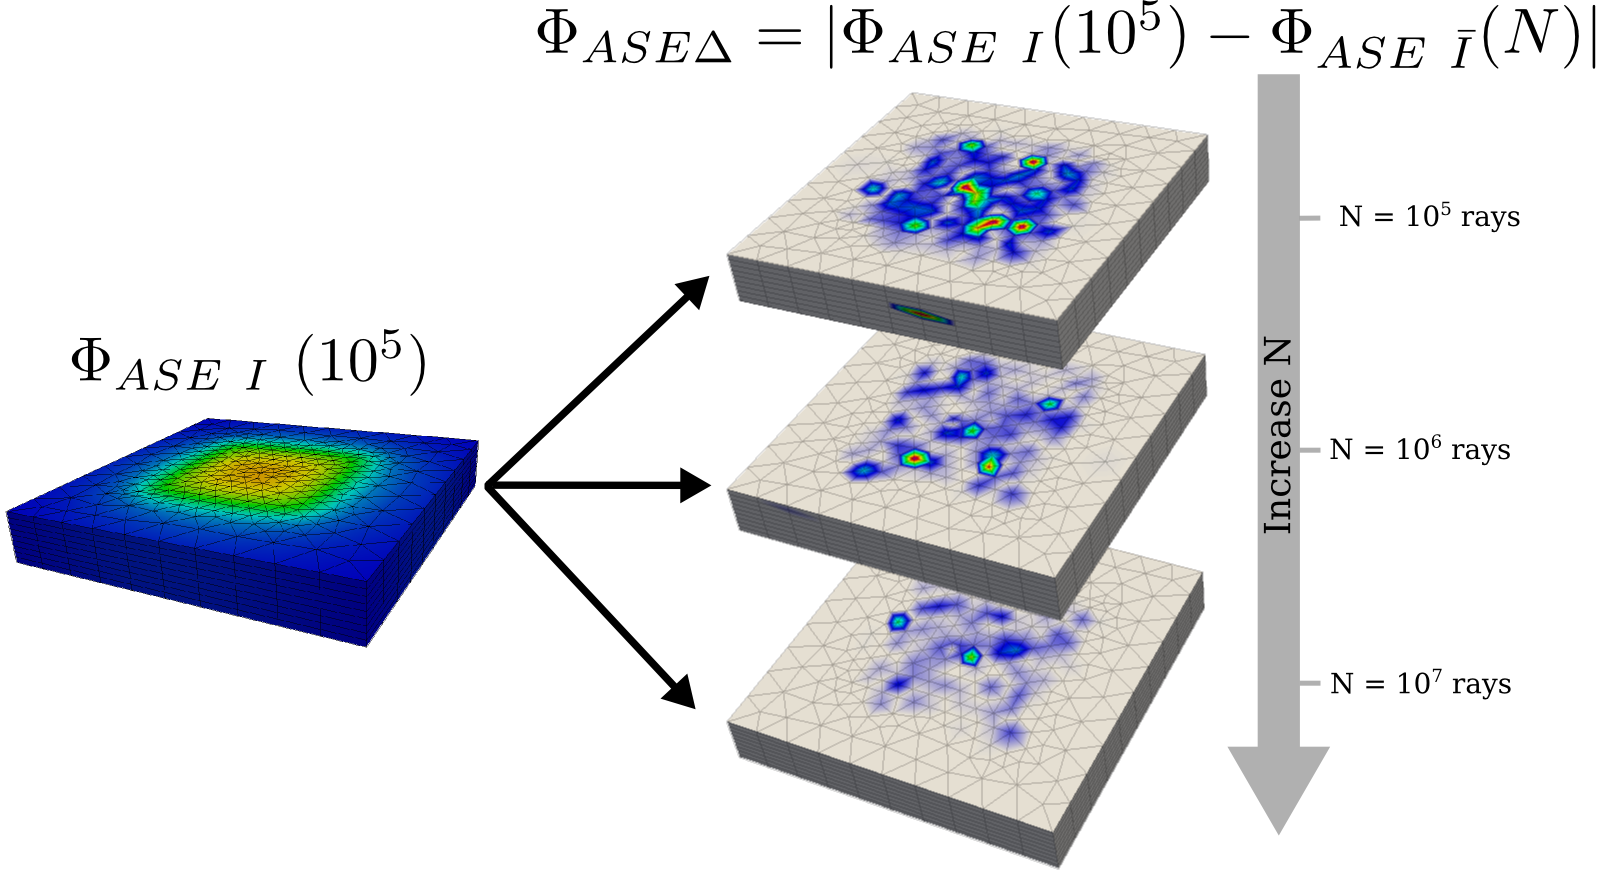
\includegraphics{graphics/phiASE_difference_new.png}}}
  \caption{$\Phi_{ASE\Delta}$ compared with increasing N}
  \label{graphic:importance}
\end{figure}

\subsection{Adaptive sampling (AS)}
\label{subsec:adaptive_sampling}
\begin{figure}[H]
  \centerline
  {\resizebox{0.5\textwidth}{!}{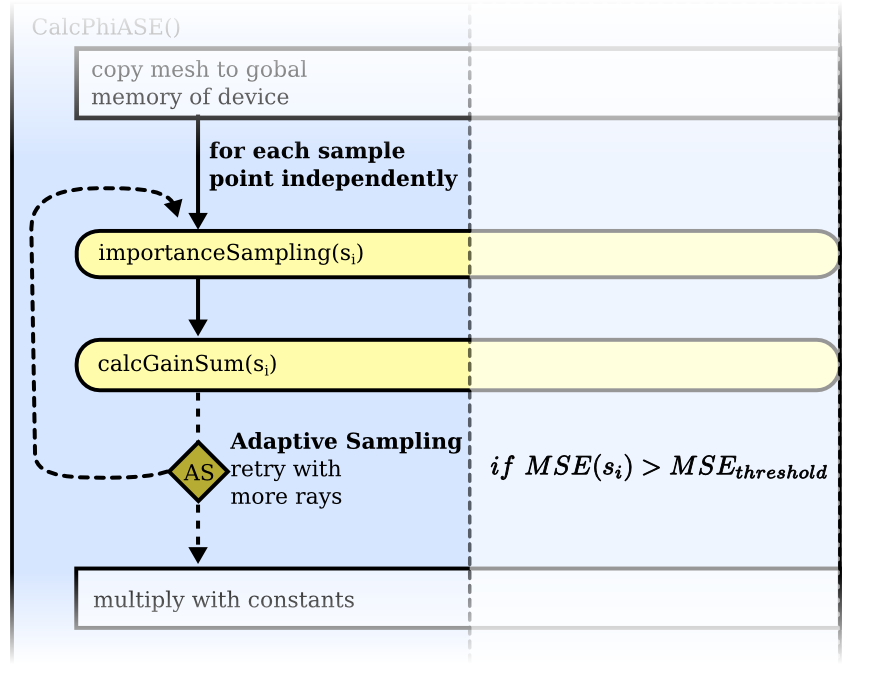
\includegraphics{graphics/PAP_step3_2.png}}}
  \caption{if the MSE is too high, both importance sampling and gain calculation
  are restarted with a higher number of rays to increase sampling resolution}
  \label{graphic:pap3}
\end{figure}
To assess the precision
and therefore the difference between the true and calculated value,
the mean squared error (MSE) is determined and serves as a core metric to
describe sampling improvements:
\begin{align}
     f(\vec{s_i}) &= \frac{1}{N} \sum_{u=0}^{N-1} gain(\overrightarrow{r_{i,u}s_i})\\
     f^2(s_i)     &= \frac{1}{N} \sum_{u=0}^{N-1} gain(\overrightarrow{r_{i,u}s_i})^2\\
     MSE(s_i)     &= \sqrt{\frac{f^2(s_i) - f(s_i)^2}{N}}
\end{align}
Since most sample points~$s_i$ have a low $MSE(s_i)$, there is no need
to sample them with a high number of rays. Only some outliers need to
be sampled with a higher resolution to reduce the occuring variance. This can be done with an adaptive
method, which allows to remove strong peaks in the result
of the simulation by resampling these points with more rays. The number of rays
is increased with each iteration, until the desired MSE threshold is met or 
a defined maximum number of rays is reached (Figure~\ref{graphic:pap3}).
Note that the importance sampling step needs to be executed again, since
the number of rays changed, leading to a slightly different distribution.

Potentially unbalanced load, caused by a varying number of rays per sample 
in a multi-GPU scenario is mitigated by the MPI load balancer (see \cref{subsubsec:multigpu}).

For comparision, the impact of importance sampling
on the MSE values is shown (see Figure~\ref{plot:importance2}). 
Importance sampling alone already reduces the MSE values for
many sample points significantly.
\begin{figure}[H]
  \centerline{
    \resizebox{0.5\textwidth}{!}{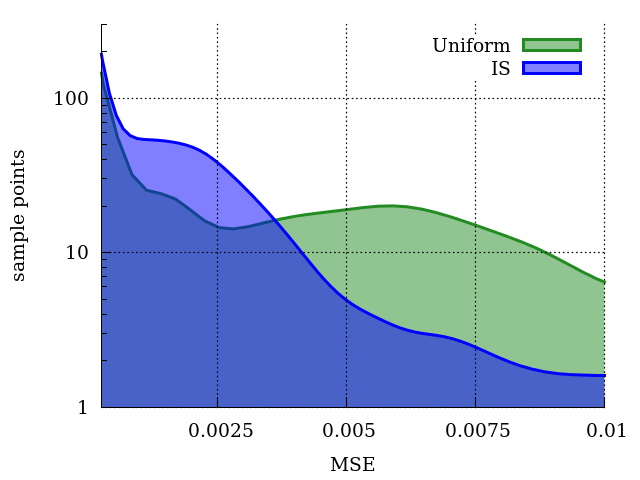
\includegraphics{plot/mse_importance.png}}}
  \caption{histogram comparing MSE values for IS sampling and Uniform sampling}
  \label{plot:importance2}
\end{figure}
By using also adaptive sampling, the MSE values are reduced to a user-defined MSE threshold.
Figure~\ref{plot:adaptive} shows the histogramm of MSE values for a MSE threshold
of $0.005$. All sample points~$s_i$ with $MSE(s_i) > 0.005$ were resampled with more rays
per sample point to lower their MSE value. The other sample points could remain unchanged.
\begin{figure}[H]
  \centerline{
    \resizebox{0.5\textwidth}{!}{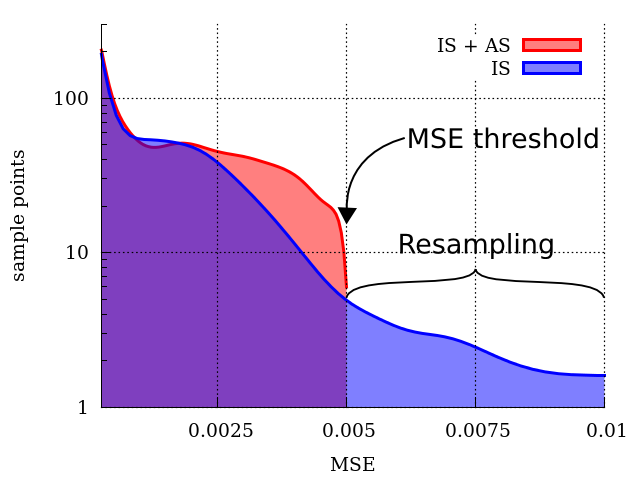
\includegraphics{graphics/mse_adaptive.png}}}
  \caption{histogram of MSE values IS and IS + AS}
  \label{plot:adaptive}
\end{figure}
The adaptive method will not reduce the average MSE over all sample points,
but it will reduce the maximal MSE values of the outliers. Thus, using the adaptive
method gives lower error and a better error distribution while maintaining
roughly the same calculation time.


\subsection{Repetitive sampling (RS)}
\begin{figure}[H]
  \centerline
  {\resizebox{0.5\textwidth}{!}{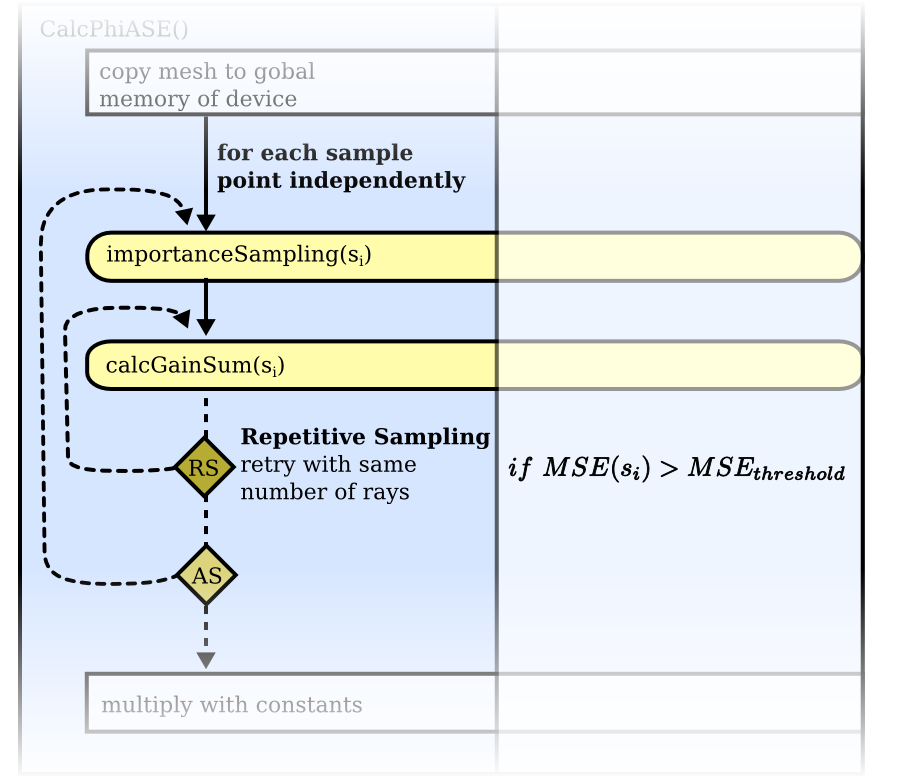
\includegraphics{graphics/PAP_step4_2.png}}}
  \caption{If the MSE is too high, gain calculation is restarted with another
    random seed and the same number of rays. The calculated importance will stay the same.}
  \label{graphic:pap4}
\end{figure}
Some outliers of the Monte-Carlo method are not related to an insufficient
sampling resolution, but rather an unlucky seed for the random number generator.
Repetitive sampling lowers the MSE values without increasing the number of rays,
by resampling the sample point with a different seed. Only after several failed attempts, it will fall back to adaptive
sampling (Figure~\ref{graphic:pap4}). This can reduce the number of rays over all sample points and therefore
also runtime. Thus, repetitive sampling is an optimization in addition to adaptive sampling. 
Note, that repetitive sampling does not require to execute the importance
sampling again (unlike adaptive sampling).

Figure~\ref{plot:repetitive} shows the sampling resolution
of the sample points in a histogram when using a MSE of 0.001. 
The AS approach alone takes about 1160s to accomplish the desired result. Simulating with RS reduces
simulations sampled with $10^8$ rays by 319 sample points, resulting in 
$3\cdot10^{10}$ rays less to calculate and a runtime of 600s to reach the threshold. Because reducing the number of rays always
reduces runtime, it explains the difference in runtime
of 560s.
\begin{figure}[H]
  \centerline{
    \resizebox{0.5\textwidth}{!}{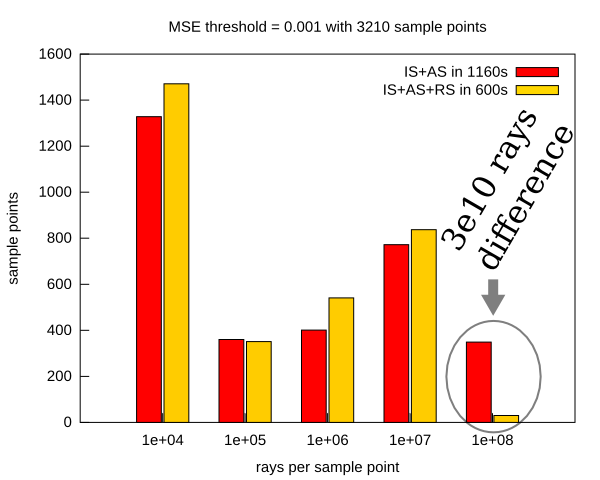
\includegraphics{graphics/repetitive_sampling.png}}}
  \caption{AS and RS compared by rays per sample point}
  \label{plot:repetitive}
\end{figure}

\subsection{Benefits of sample methods}
In this section, the presented methods IS, AS and RS are compared by runtime
and precision.
In Figure~\ref{graphic:methods_compare}, the time to reach an
MSE value of 0.01 was measured. It is evident that AS and RS perform
much better than Uniform or IS. 
\begin{figure}[H]
  \centerline{
    \resizebox{0.5\textwidth}{!}{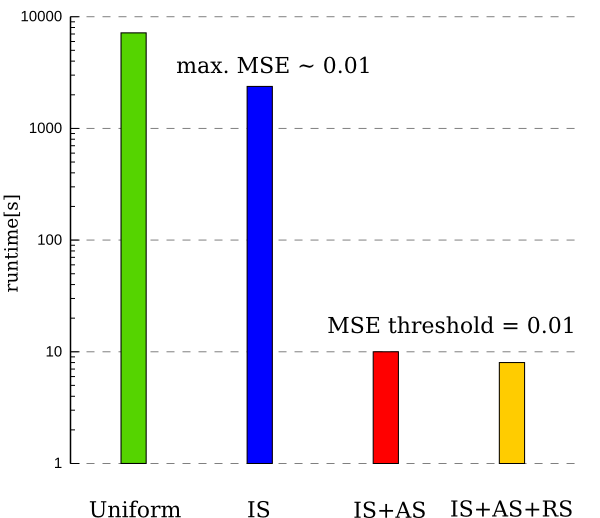
\includegraphics{graphics/methods_compare.png}}}
  \caption{Methods with same MSE value}
  \label{graphic:methods_compare}
\end{figure}
Figure~\ref{graphic:methods_compare2} shows the maximal MSE values
of the gain medium for a fixed runtime of 10s. Uniform and IS 
produce higher maxima than AS or RS.
\begin{figure}[H]
  \centerline{
    \resizebox{0.5\textwidth}{!}{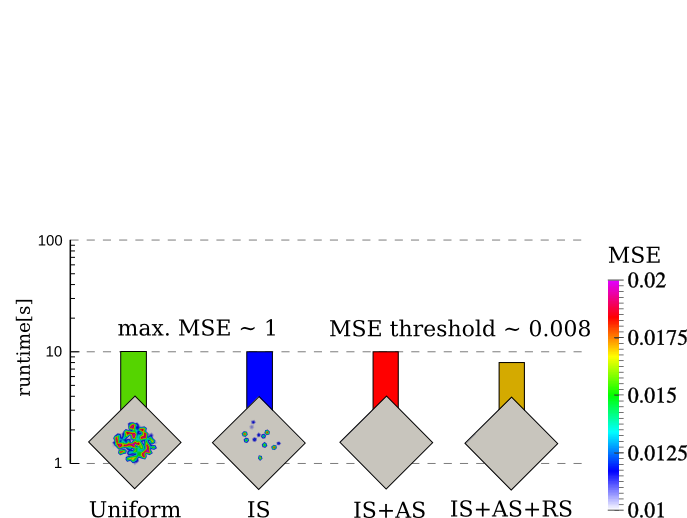
\includegraphics{graphics/methods_compare2.png}}}
  \caption{max. MSE values for a fixed runtime of 10s}
  \label{graphic:methods_compare2}
\end{figure}
